\subsection{水平放置的平面图形的直观图的画法}\label{subsec:1-3}

\begin{enhancedline}

\begin{wrapfigure}[8]{r}{4cm}
    \centering
    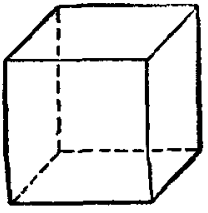
\includegraphics[width=3cm]{../pic/ltjh-ch1-08.png}
    \caption{}\label{fig:ltjh-1-8}
\end{wrapfigure}

把空间图形画在纸上或黑板上,这就是用一个平面图形来表示空间图形。
这样的平面图形不是空间图形的真实形状,而是它的直观图。
如图 \ref{fig:ltjh-1-8} 是正方体的一种直观图。
正方体的各个面本来都是正方形,但是在直观图中,有一些面画成了平行四边形,
虽然直观图是和空间图形不同的平面图形,但它有较强的立体感。

要画空间图形的直观图,首先要学会水平放置的平面图形的直观图的画法。
下面举例说明一种常用的画法。


\liti 画水平放置的正六边形的直观图(图 \ref{fig:ltjh-1-9})。

\begin{figure}[htbp]
    \centering
    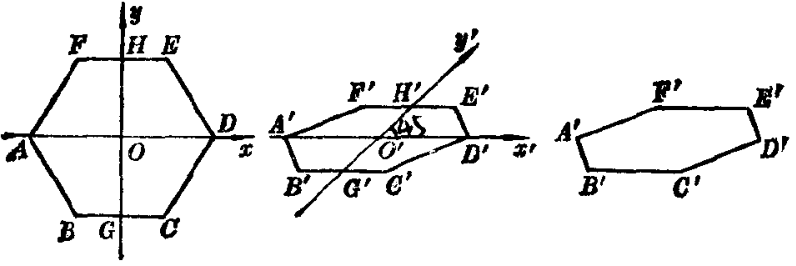
\includegraphics[width=11cm]{../pic/ltjh-ch1-09.png}
    \caption{}\label{fig:ltjh-1-9}
\end{figure}

\huafa (1) 在已知正六边形 $ABCDEF$ 中,取对角线 $AD$ 所在的直线为 $x$轴,取对称轴 $GH$ 为 $y$ 轴。
画对应的 $x'$ 轴、$y'$ 轴, 使 $\angle x'O'y' = 45^\circ$。

(2) 以点 $O'$ 为中点,在 $x'$ 轴上取 $A'D' = AD$, 在 $y'$ 轴上取 $G'H' = \exdfrac{1}{2} GH$。
以点 $H'$ 为中点画 $F'E'$ 平行于 $x'$ 轴,并等于 $FE$;
再以 $G'$ 为中点画 $B'C'$ 平行于 $x'$ 轴,并等于 $BC$。

(3) 连结 $A'B'$、$C'D'$、$D'E'$、$F'A'$。所得的六边形 $A'B'C'D'E'F'$ 就是正六边形 $ABCDEF$ 的直观图。

\zhuyi 图画好后,要擦去辅助线 \footnotemark 。
\footnotetext{辅助线包括 $x'$ 轴、$y'$ 轴及为画图添加的线。}

上面画直观图的方法叫做\zhongdian{斜二测画法},这种画法的规则是:

(1)\zhongdian{在已知图形中取互相垂直的轴 $\bm{Ox}$、$\bm{Oy}$。
画直观图时,把它画成对应的轴 $\bm{O'x'}$、$\bm{O'y'}$,
使 $\bm{\angle x'O'y' = 45^\circ}$(或 $\bm{135^\circ}$)。}
它们确定的平面表示水平平面。

(2)\zhongdian{已知图形中平行于 $\bm{x}$ 轴或 $\bm{y}$ 轴的线段,在直观图中分别画成平行于 $\bm{x'}$ 轴或 $\bm{y'}$ 轴的线段。}

(3)\zhongdian{已知图形中平行于 $\bm{x}$ 轴的线段,在直观图中保持原长度不变;
平行于 $\bm{y}$ 轴的线段,长度为原来的一半。}


\liti 画水平放置的正五边形的直观图(图 \ref{fig:ltjh-1-10})。

\begin{figure}[htbp]
    \centering
    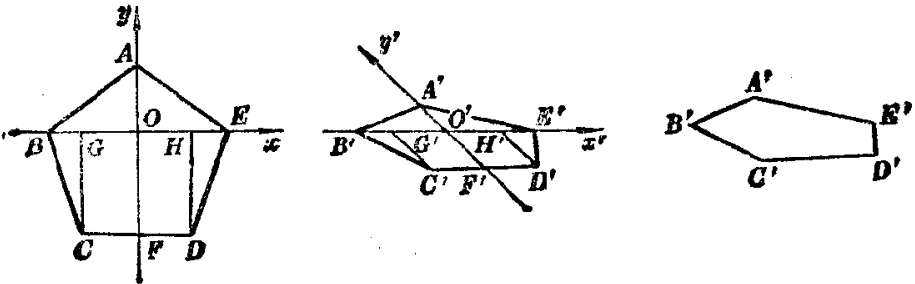
\includegraphics[width=11cm]{../pic/ltjh-ch1-10.png}
    \caption{}\label{fig:ltjh-1-10}
\end{figure}

\huafa(1) 在已知正五边形 $ABCDE$ 中,取对角线 $BE$ 所在的直线为 $x$ 轴,取对称轴 $AF$ 为 $y$ 轴。
分别过点 $C$、$D$ 作 $CG \pingxing Oy$、$DH \pingxing Oy$,与 $x$ 轴分别交于 $G$、$H$。
画对应的 $x'$ 轴、$y'$ 轴,使 $\angle x'O'y' = 135^\circ$。

(2) 以点 $O'$ 为中点,在 $x'$ 轴上截取 $G'H' = GH$。
在 $x'$ 轴的同一侧画线段 $C'G' \pingxing O'y'$、$D'H' \pingxing O'y'$,
并使 $C'G'= \exdfrac{1}{2} CG$, $D'H' = \exdfrac{1}{2} DH$;
在 $x'$ 轴的另一侧的 $y'$ 轴上取一点 $A'$,使 $O'A' = \exdfrac{1}{2} OA$;
以点 $O'$ 为中点,在 $x'$ 轴上截取 $B'E' = BE$。

(3) 连结 $A'B'$、$B'C'$、$C'D'$、$D'E'$、$E'A'$。
所得的五边形 $A'B'C'D'E'$ 就是正五边形 $ABCDE$ 的直观图。



\begin{lianxi}

% TODO: wrapfigure 在这里无法正常使用
\begin{minipage}{10cm}
    \xiaoti{画水平放置的正方形、正三角形的直观图。}

    \xiaoti{图中所给出的 $x$ 轴、$y$ 轴经过正五边形中心,画这个正五边形的直观图。}
\end{minipage}
\quad
\begin{minipage}{4cm}
    \centering
    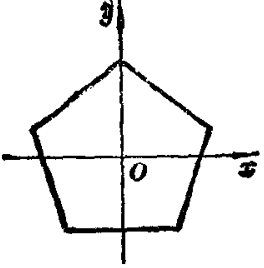
\includegraphics[width=3cm]{../pic/ltjh-ch1-subsec3-lx-02.png}\\
    (第 2 题)
\end{minipage}

\end{lianxi}
\end{enhancedline}
